% Typeset version of the agent-written analysis note
% notes/kstll_note_agent_v3.md (accepted by the AI note referee).
% The text and all numbers are the agent's; this file only adds LaTeX
% typography (math notation, booktabs tables, figure floats, captions).
% Compile: xelatex (twice, for the table of contents).
\documentclass[11pt]{article}
\usepackage[margin=1in]{geometry}
\usepackage{amsmath,amssymb}
\usepackage{booktabs}
\usepackage{graphicx}
\usepackage{caption}
\usepackage[colorlinks=true,linkcolor=blue!50!black,citecolor=blue!50!black,urlcolor=blue!50!black]{hyperref}
\usepackage{xcolor}
\captionsetup{font=small,labelfont=bf,width=0.92\textwidth}
\graphicspath{{figures/}}
\setkeys{Gin}{width=0.72\textwidth}
\emergencystretch=2em

\newcommand{\BF}{\mathcal{B}}
\newcommand{\Kst}{K^{*0}}
\newcommand{\Mbc}{M_{\mathrm{bc}}}
\newcommand{\dE}{\Delta E}
\newcommand{\mll}{m_{\ell\ell}}
\newcommand{\jpsi}{J/\psi}

\title{Sensitivity study: $B^0 \to \Kst(K^{+}\pi^{-})\,\ell^{+}\ell^{-}$
  with a $\jpsi\,\Kst$ peaking background}
\author{K.~Yoshihara (University of Hawai\textquoteleft i at M\=anoa)\\[2pt]
  \small analysis performed and written by an LLM agent (Claude) under
  human review;\\ \small typeset from the agent's approved Markdown note}
\date{v1.1 --- September 19, 2026}

\begin{document}
\maketitle

\begin{center}
\fbox{\parbox{0.9\textwidth}{\small
This study uses only publicly available tools and publications. No
Belle~II internal materials --- data, MC, internal notes, or the software
framework --- are used. Everything is open-source and runs on a laptop.}}
\end{center}

\begin{abstract}
Using existing fast-simulation ntuples (10000 generated
$B^0\to\Kst\ell^{+}\ell^{-}$ signal events and 5000 generated
$B^0\to\jpsi(\to\ell^{+}\ell^{-})\Kst$ background events, split evenly
between $e^+e^-$ and $\mu^+\mu^-$), we apply the Belle/Belle~II
$B\to K^{*}(892)\ell^{+}\ell^{-}$ selection: a $K\pi$ mass window
($0.896 \pm 0.075$\,GeV), $\Mbc > 5.27$\,GeV, an asymmetric per-flavor
$\dE$ window, and an asymmetric charmonium veto in $\mll$. Before the
veto the $\jpsi\,\Kst$ control region is essentially pure background
(20645 $e^+e^-$ and 19132 $\mu^+\mu^-$ events at 1\,ab$^{-1}$, purity
99.89\%); after the veto the leakage drops to 43.2 events ($e^+e^-$) and
consistent with zero, 68\%-CL upper limit $\sim$25 events
($\mu^+\mu^-$), a signal-efficiency step of 92.5\% versus a background
rejection of 99.8--100\%. At 1\,ab$^{-1}$ the projected yields are 285.7
$e^+e^-$ and 251.8 $\mu^+\mu^-$ signal candidates, giving $\sim$6.3\%
relative statistical precision per flavor and 4.5\% combined. Continuum
and generic-$B\bar B$ combinatorial background are not modeled in this
study.
\end{abstract}

\tableofcontents

\section{Introduction}

$B^0\to\Kst\ell^{+}\ell^{-}$ ($\ell = e,\mu$) is a
flavor-changing-neutral-current $b\to s\,\ell^{+}\ell^{-}$ transition,
forbidden at tree level in the Standard Model and sensitive to new heavy
particles in the loop. Belle first measured its branching fraction and
forward-backward asymmetry using the beam-energy-constrained mass
$\Mbc$, the energy difference $\dE$, and a $K\pi$ invariant-mass window
around the $K^{*}(892)$, with asymmetric charmonium ($\jpsi$,
$\psi(2S)$) vetoes in the dilepton mass that are wider on the low side
for electrons because of bremsstrahlung (Wei et al.\ [Belle], PRL 103,
171801 (2009)). The vetoed $\jpsi\,K^{*}$ sample itself served as the
control channel for efficiencies and PID. The most recent Belle~II
measurement of this same final state (arXiv:2206.05946) uses the
identical strategy and quotes explicit numerical veto windows, $\jpsi$
excluded at $M(\mu^+\mu^-) \notin [2.946, 3.176]$\,GeV and
$M(e^+e^-) \notin [2.846, 3.176]$\,GeV, which this note adopts as the
starting point and validates on its own simulation.

This note reproduces that selection logic on a fast-simulation sample to
estimate the signal yield and statistical precision achievable with
1\,ab$^{-1}$, and to quantify the size and control-region purity of the
residual $\jpsi\,\Kst$ peaking background after the veto. Continuum and
generic-$B\bar B$ combinatorial background are explicitly \textbf{not}
modeled in this study (no such samples were generated); this is stated
wherever it matters and discussed in Section~\ref{sec:discussion}.

\section{Data samples and analysis tools}
\label{sec:samples}

Samples were \textbf{not regenerated} for this study; two existing
ntuples (produced by the script \texttt{make\_ntuple\_exclusive.py},
one row per reconstructed $B$ candidate) were used directly.

\begin{table}[htbp]
\centering\footnotesize
\setlength{\tabcolsep}{4pt}
\resizebox{\textwidth}{!}{%
\begin{tabular}{llllll}
\toprule
Sample & Process & Generator model & Events & Flavor split & Seeds \\
\midrule
sig\_kstll.root & $B^0\to\Kst(K^{+}\pi^{-})\ell^{+}\ell^{-}$ & EvtGen \texttt{BTOSLLBALL} & 10000 & 50\% $ee$, 50\% $\mu\mu$ & 32 / 33 \\
bkg\_jpsikst.root & $B^0\to\jpsi(\to\ell\ell)\Kst(K^{+}\pi^{-})$ & EvtGen ($\jpsi K^{*}$ + $\jpsi\to\ell\ell$) & 5000 & 50\% $ee$, 50\% $\mu\mu$ & 34 / 35 \\
\bottomrule
\end{tabular}}
\caption{MC samples used in this study.}
\label{tab:samples}
\end{table}

Relevant branches: \texttt{m\_visible} (reconstructed $m(K\pi)$, i.e.\
the $K^{*}$ candidate mass), \texttt{mbc}, \texttt{delta\_e},
\texttt{m\_ll} (reconstructed dilepton mass), \texttt{lep\_flavor}
(11 = $e$, 13 = $\mu$). These ntuples carry no \texttt{true\_mode}
branch (unlike the \texttt{make\_ntuple} output used in other notes of
this framework): truth information here is simply which file a candidate
came from.

The events were passed through the framework's fast detector simulation
(track/cluster smearing, lepton and hadron PID) at ntuple-production
time; only $\sim$44--54\% of generated events per flavor yield a
reconstructed candidate row in the ntuple
(Section~\ref{sec:cutflow}, ``reconstructed'' cutflow stage) --- this
already includes basic reconstruction/acceptance losses.

\textbf{Normalization to 1\,ab$^{-1}$.} The number of available
$B^0/\bar B^0$ mesons is
\begin{equation*}
N(B^0\ \text{avail})
 = 2 \times f_{00} \times \sigma(B\bar B) \times L
 = 2 \times 0.486 \times 1.1\,\text{nb} \times 10^{9}\,\text{nb}^{-1}
 = 1.0692\times 10^{9}
\end{equation*}
using $f_{00} = 0.486$, $\sigma(B\bar B) = 1.1$\,nb, and
$L = 1\,\text{ab}^{-1} = 10^{9}\,\text{nb}^{-1}$. Per-event luminosity
weights (expected events at 1\,ab$^{-1}$ per generated MC event, by
flavor) are
\begin{equation*}
w = \frac{N(B^0\ \text{avail}) \times \BF(\text{mode}) \times
          \BF(\Kst\to K^{+}\pi^{-})}{N_{\mathrm{generated}}(\text{flavor})}
\end{equation*}
with $\BF(\Kst ee) = 1.03\times 10^{-6}$,
$\BF(\Kst\mu\mu) = 1.05\times 10^{-6}$,
$\BF(\Kst\to K^{+}\pi^{-}) = 2/3$,
$\BF(\jpsi\,\Kst) = 1.27\times 10^{-3}$,
$\BF(\jpsi\to\ell\ell) = 0.0597$ (same for $e$ and $\mu$), and
$N_{\mathrm{generated}} = 5000$ per signal flavor, 2500 per background
flavor:

\begin{table}[htbp]
\centering
\begin{tabular}{lr}
\toprule
 & $w$ (events / 1\,ab$^{-1}$ per generated MC event) \\
\midrule
signal, $e^+e^-$ & 0.1468 \\
signal, $\mu^+\mu^-$ & 0.1497 \\
$\jpsi\,\Kst$, $e^+e^-$ & 21.618 \\
$\jpsi\,\Kst$, $\mu^+\mu^-$ & 21.618 \\
\bottomrule
\end{tabular}
\caption{Per-event luminosity weights.}
\label{tab:weights}
\end{table}

The huge weight of the $\jpsi\,\Kst$ sample reflects
$\BF(\jpsi\,\Kst)$ being $\sim$1000$\times$ larger than the signal BF:
the charmonium veto (Section~\ref{sec:veto}) must reject this background
very efficiently.

All figures were produced with \texttt{plot\_stacked}
(luminosity-weighted, truth-split by sample and, where relevant, by
reconstructed lepton flavor via a \texttt{lep\_flavor} selection). All
cut values were fixed with the \texttt{scan\_cut} tool, scanning one
variable at a time on top of the preceding cuts, using unweighted MC
counts as the figure of merit $S/\sqrt{S+B}$ (a shape-level proxy; the
weighted, physical yields are computed separately in
Section~\ref{sec:results}).

\section{Event selection}

Four sequential cuts are applied, in the same order and with the same
physics motivation as Wei et al.\ [Belle] and the Belle~II
$K^{*}(892)\ell\ell$ measurement.

\subsection{\texorpdfstring{$K^{*}$ mass window ($m_{\mathrm{visible}}$)}{K* mass window (m\_visible)}}

\emph{Targets:} wrong-mass $K$--$\pi$ combinations under the
$K^{*}(892)$ lineshape (natural width 47\,MeV) folded with detector
resolution. In this simplified simulation both the signal and the
$\jpsi\,\Kst$ background contain a genuine $K^{*}(892)$, so this cut is
a resolution/acceptance cut rather than a signal/background discriminant
--- as confirmed by the scan, where the FOM falls monotonically as the
window is tightened for both samples equally (\texttt{scan\_cut} on
\texttt{m\_visible}, symmetric window):

\begin{table}[htbp]
\centering
\begin{tabular}{lrr}
\toprule
window (GeV) & signal eff. & background eff. \\
\midrule
$\pm 0.05$ & 74.8\% & 75.7\% \\
$\boldsymbol{\pm 0.075}$ \textbf{(chosen)} & \textbf{83.6\%} & \textbf{83.7\%} \\
$\pm 0.10$ & 87.8\% & 88.4\% \\
\bottomrule
\end{tabular}
\caption{Scan of the symmetric $K^{*}$ mass window.}
\label{tab:scan_kst}
\end{table}

Window chosen: $\mathbf{0.821 < m(K\pi) < 0.971}$\,\textbf{GeV}
($0.896 \pm 0.075$\,GeV), retaining $\sim$84\% of both samples while
removing the far tails where a real combinatorial background (not
modeled here) would dominate. Figure~\ref{fig:mvisible} shows the
distribution with cut lines at the window edges.

\begin{figure}[htbp]
\centering
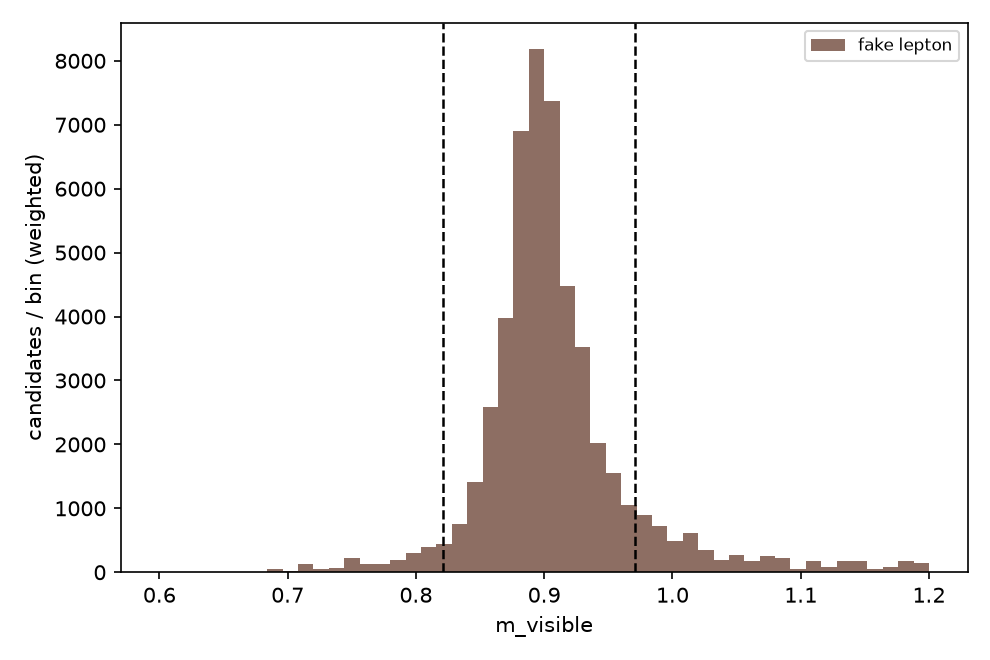
\includegraphics{01_mvisible_presel.png}
\caption{Reconstructed $K\pi$ invariant mass ($K^{*}$ candidate mass)
before any selection, stacked by sample (luminosity-weighted); the
vertical lines mark the chosen $0.821 < m(K\pi) < 0.971$\,GeV window.}
\label{fig:mvisible}
\end{figure}

\subsection{\texorpdfstring{Beam-energy-constrained mass ($\Mbc$)}{Beam-energy-constrained mass (Mbc)}}

\emph{Targets:} combinatorial/continuum background populating low
$\Mbc$ (not modeled here) and mis-reconstructed candidates; real signal
peaks at the beam energy. Scan on top of the $K^{*}$ window
(\texttt{scan\_cut}, \texttt{mbc}, direction ``$>$''):

\begin{table}[htbp]
\centering
\begin{tabular}{lrrr}
\toprule
$\Mbc >$ (GeV) & $S$ & $B$ & $S/\sqrt{S+B}$ \\
\midrule
5.24 & 4103 & 1960 & 52.7 \\
5.26 & 4048 & 1931 & 52.4 \\
\textbf{5.27 (chosen)} & \textbf{3999} & \textbf{1900} & \textbf{52.1} \\
5.275 & 3953 & 1875 & 51.8 \\
5.28 & 860 & 425 & 24.0 \\
\bottomrule
\end{tabular}
\caption{Scan of the $\Mbc$ requirement on top of the $K^{*}$ window.}
\label{tab:scan_mbc}
\end{table}

The sharp drop above 5.28\,GeV marks the edge of the $\Mbc$ peak itself
(beam-energy edge, $\sim$5.29\,GeV, smeared by detector resolution);
cutting there would remove signal, not background.
$\boldsymbol{\Mbc > 5.27}$\,\textbf{GeV} is chosen, following Wei et
al., retaining 96\% of the $K^{*}$-window sample.
Figure~\ref{fig:mbc} shows the distribution with the cut line at
5.27\,GeV.

\begin{figure}[htbp]
\centering
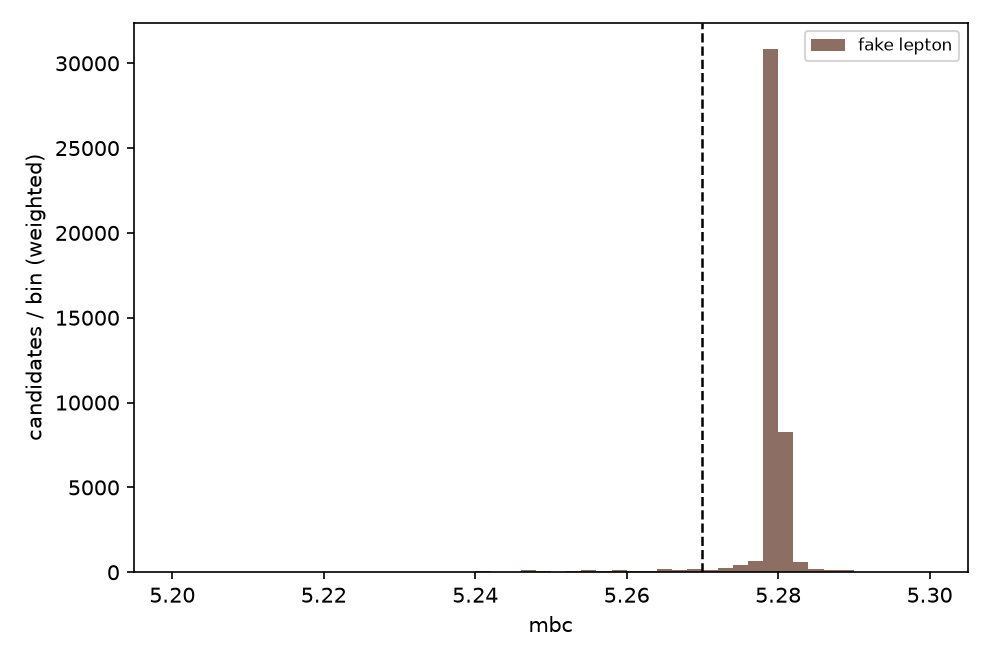
\includegraphics{02_mbc_afterkst.png}
\caption{Beam-energy-constrained mass $\Mbc$ after the $K^{*}$ mass
window, stacked by sample (luminosity-weighted); the vertical line marks
the $\Mbc > 5.27$\,GeV requirement.}
\label{fig:mbc}
\end{figure}

\subsection{\texorpdfstring{Energy difference ($\dE$), per lepton flavor}{Energy difference (Delta E), per lepton flavor}}

\emph{Targets:} partially reconstructed or extra-energy background; for
electrons the signal itself develops a low-side tail from final-state
bremsstrahlung not fully recovered by clustering, motivating an
asymmetric, wider low-side window (as in Wei et al.). Scans on top of
the $K^{*}$+$\Mbc$ selection, separately per flavor (\texttt{scan\_cut},
\texttt{delta\_e}):

Electron channel (lower edge, direction ``$>$''): FOM rises
monotonically as the window is loosened and plateaus around $-0.25$ to
$-0.30$\,GeV (38.0--38.2), while the upper edge saturates at
$+0.05$\,GeV ($S$ stops increasing beyond that). Chosen:
$\mathbf{-0.25 < \dE < 0.05}$\,\textbf{GeV}.

Muon channel: the same scan shows a much smaller low-side tail (FOM
35.2--35.3 essentially flat from $-0.10$ to $-0.30$\,GeV), consistent
with the absence of bremsstrahlung; the upper edge again saturates at
$+0.05$\,GeV. Chosen: $\mathbf{-0.10 < \dE < 0.05}$\,\textbf{GeV}, a
narrower low side than for electrons, reproducing the qualitative
asymmetry reported by Wei et al.

Figures~\ref{fig:deltae_ee} and \ref{fig:deltae_mumu} show the
distributions with cut lines at the chosen edges.

\begin{figure}[htbp]
\centering
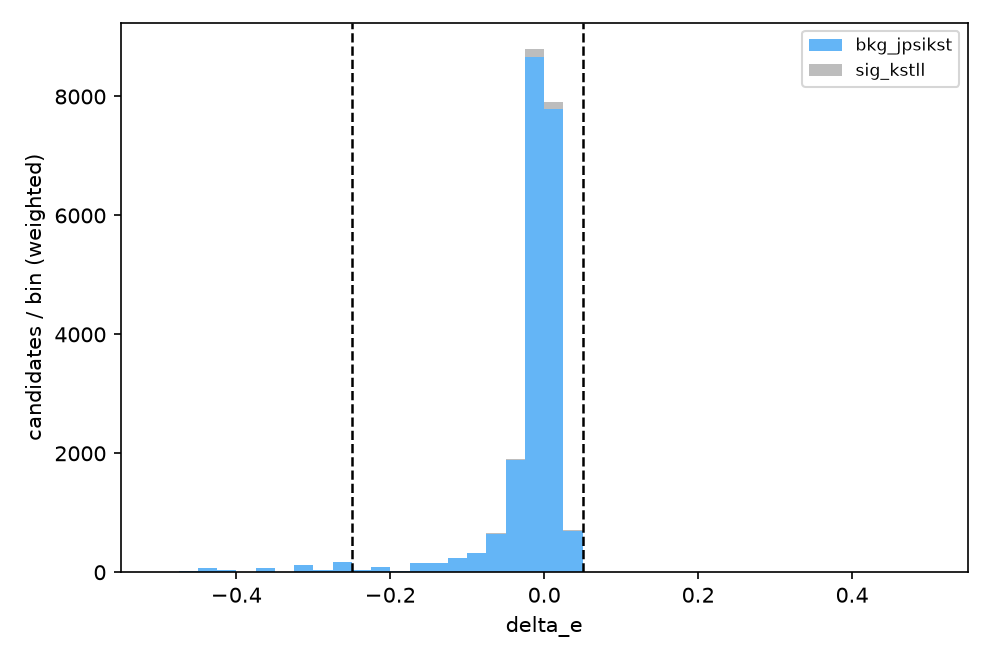
\includegraphics{03_deltae_ee.png}
\caption{Energy difference $\dE$ in the electron channel after the
$K^{*}$ and $\Mbc$ requirements, stacked by sample
(luminosity-weighted); the vertical lines mark the asymmetric
$-0.25 < \dE < 0.05$\,GeV window, wider on the low side because of
bremsstrahlung.}
\label{fig:deltae_ee}
\end{figure}

\begin{figure}[htbp]
\centering
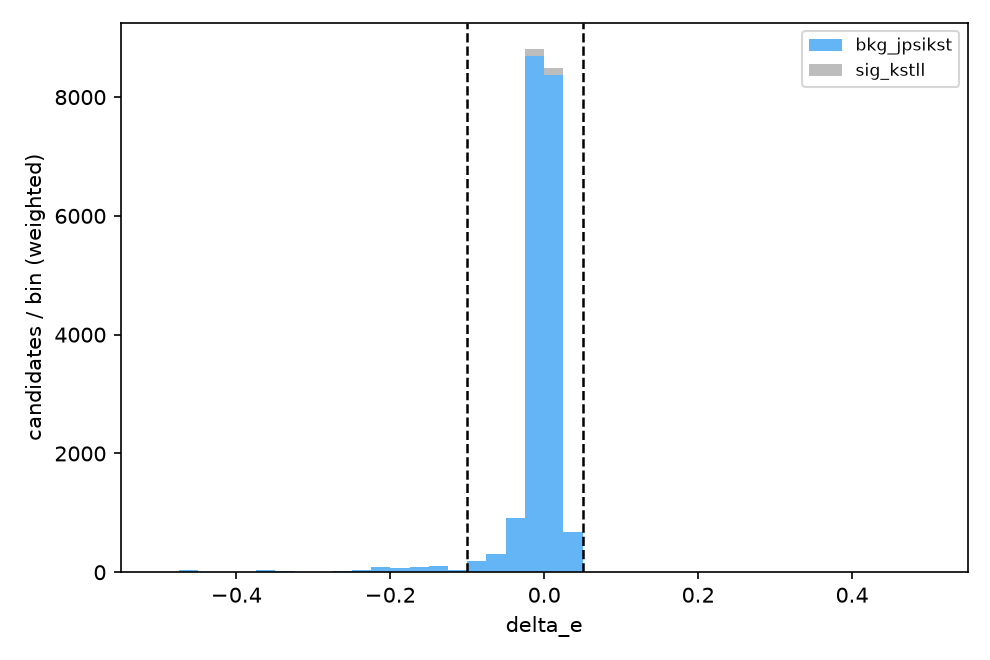
\includegraphics{03_deltae_mumu.png}
\caption{Energy difference $\dE$ in the muon channel after the $K^{*}$
and $\Mbc$ requirements, stacked by sample (luminosity-weighted); the
vertical lines mark the narrower $-0.10 < \dE < 0.05$\,GeV window.}
\label{fig:deltae_mumu}
\end{figure}

\subsection{\texorpdfstring{Charmonium ($\jpsi$) veto in $\mll$, asymmetric per flavor}{Charmonium (J/psi) veto in m\_ll, asymmetric per flavor}}
\label{sec:veto}

\emph{Targets:} $B^0\to\jpsi(\to\ell^{+}\ell^{-})\Kst$, the dominant
peaking background, $\sim$1000$\times$ the signal rate before any veto.
The trade-off scan (\texttt{scan\_cut}, \texttt{m\_ll}, on top of
$K^{*}$+$\Mbc$+$\dE$, per flavor) brackets the peak from below and
above:

Electron channel, lower edge (keep $\mll <$ threshold): background
stays at 0--2 events up to 2.9\,GeV then rises quickly (11 at 2.95, 30
at 3.0). Upper edge (keep $\mll >$ threshold): background jumps from 297
($>3.10$, inside the radiative tail region) to 4 ($>3.13$) to 0
($\geq 3.15$).

Muon channel, lower edge: background is 0 up to 2.98\,GeV, then rises
(7 at 3.02, 26 at 3.05). Upper edge: background jumps from 316
($>3.10$) to 1 ($>3.13$) to 0 ($\geq 3.15$).

Both flavors therefore have a ``safe'' plateau (background $\sim$0,
signal near its local maximum) that brackets the Belle~II window values;
these are adopted as the final veto, confirmed rather than re-derived by
the scan:

\begin{table}[htbp]
\centering
\begin{tabular}{ll}
\toprule
flavor & veto window (excluded) \\
\midrule
$e^+e^-$ & 2.846 -- 3.176\,GeV \\
$\mu^+\mu^-$ & 2.946 -- 3.176\,GeV \\
\bottomrule
\end{tabular}
\caption{Adopted charmonium veto windows in $\mll$ (Belle~II,
arXiv:2206.05946).}
\label{tab:veto}
\end{table}

Figures~\ref{fig:mll_ee} and \ref{fig:mll_mumu} show the dilepton-mass
distributions with the veto windows.

\begin{figure}[htbp]
\centering
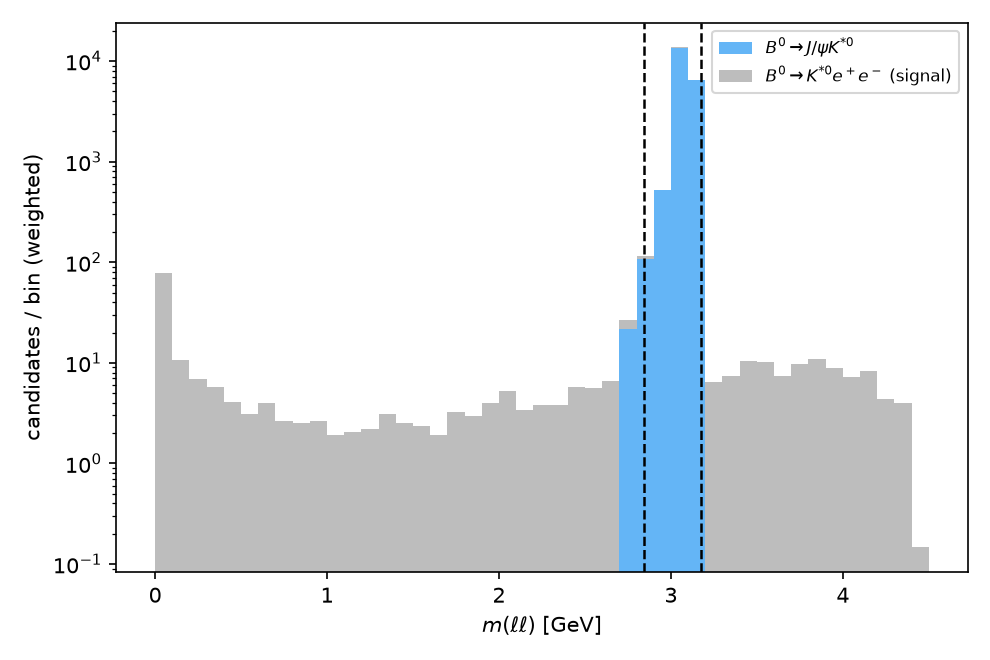
\includegraphics{04_mll_ee_veto.png}
\caption{Dilepton mass $\mll$ in the electron channel after the $K^{*}$,
$\Mbc$ and $\dE$ requirements, stacked by sample (luminosity-weighted);
the vertical lines mark the asymmetric $\jpsi$ veto window
$[2.846, 3.176]$\,GeV, wider on the low side because of the
bremsstrahlung tail.}
\label{fig:mll_ee}
\end{figure}

\begin{figure}[htbp]
\centering
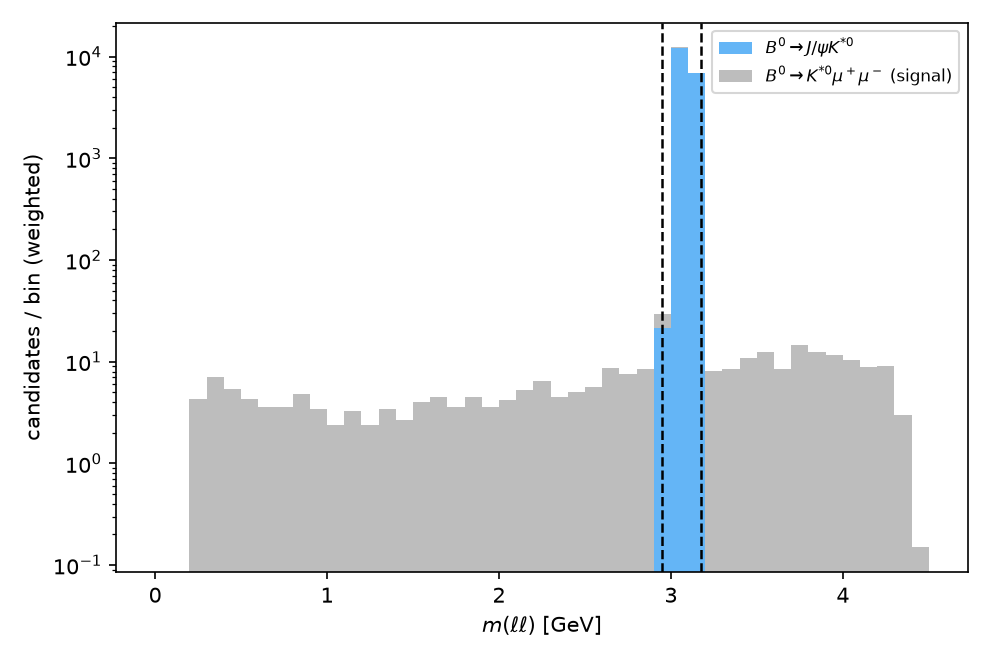
\includegraphics{04_mll_mumu_veto.png}
\caption{Dilepton mass $\mll$ in the muon channel after the $K^{*}$,
$\Mbc$ and $\dE$ requirements, stacked by sample (luminosity-weighted);
the vertical lines mark the $\jpsi$ veto window $[2.946, 3.176]$\,GeV.}
\label{fig:mll_mumu}
\end{figure}

\section{Full cutflow (per flavor, per sample)}
\label{sec:cutflow}

Efficiencies are cumulative relative to the number of
\textbf{generated} events for that flavor (5000 for signal, 2500 for
$\jpsi\,\Kst$ background); ``reconstructed'' is the fast-sim
reconstruction/acceptance stage already built into the ntuple.

\begin{table}[htbp]
\centering
\begin{tabular}{lrrr}
\toprule
stage & $N$ & step eff. & cum.\ eff. \\
\midrule
generated & 5000 & --- & 100.0\% \\
reconstructed & 2701 & 54.0\% & 54.0\% \\
$K^{*}$ window & 2268 & 84.0\% & 45.4\% \\
$\Mbc > 5.27$ & 2138 & 94.3\% & 42.8\% \\
$\dE$ window & 2104 & 98.4\% & 42.1\% \\
$\jpsi$ veto & 1946 & 92.5\% & $\mathbf{38.9 \pm 0.7\%}$ \\
\bottomrule
\end{tabular}
\caption{Signal cutflow, $B^0\to\Kst e^+e^-$ (5000 generated).}
\label{tab:cutflow_sig_ee}
\end{table}

\begin{table}[htbp]
\centering
\begin{tabular}{lrrr}
\toprule
stage & $N$ & step eff. & cum.\ eff. \\
\midrule
generated & 5000 & --- & 100.0\% \\
reconstructed & 2292 & 45.8\% & 45.8\% \\
$K^{*}$ window & 1907 & 83.2\% & 38.1\% \\
$\Mbc > 5.27$ & 1861 & 97.6\% & 37.2\% \\
$\dE$ window & 1819 & 97.7\% & 36.4\% \\
$\jpsi$ veto & 1682 & 92.5\% & $\mathbf{33.6 \pm 0.7\%}$ \\
\bottomrule
\end{tabular}
\caption{Signal cutflow, $B^0\to\Kst\mu^+\mu^-$ (5000 generated).}
\label{tab:cutflow_sig_mumu}
\end{table}

\begin{table}[htbp]
\centering
\begin{tabular}{lrrr}
\toprule
stage & $N$ & step eff. & cum.\ eff. \\
\midrule
generated & 2500 & --- & 100.0\% \\
reconstructed & 1295 & 51.8\% & 51.8\% \\
$K^{*}$ window & 1068 & 82.5\% & 42.7\% \\
$\Mbc > 5.27$ & 986 & 92.3\% & 39.4\% \\
$\dE$ window & 957 & 97.1\% & 38.3\% \\
$\jpsi$ veto & 2 & 0.2\% & $\mathbf{0.08 \pm 0.06\%}$ \\
\bottomrule
\end{tabular}
\caption{Background cutflow, $B^0\to\jpsi(\to e^+e^-)\Kst$
(2500 generated).}
\label{tab:cutflow_bkg_ee}
\end{table}

\begin{table}[htbp]
\centering
\begin{tabular}{lrrr}
\toprule
stage & $N$ & step eff. & cum.\ eff. \\
\midrule
generated & 2500 & --- & 100.0\% \\
reconstructed & 1101 & 44.0\% & 44.0\% \\
$K^{*}$ window & 938 & 85.2\% & 37.5\% \\
$\Mbc > 5.27$ & 914 & 97.4\% & 36.6\% \\
$\dE$ window & 885 & 96.8\% & 35.4\% \\
$\jpsi$ veto & 0 & 0.0\% & \textbf{0.0\% (0/2500)} \\
\bottomrule
\end{tabular}
\caption{Background cutflow, $B^0\to\jpsi(\to\mu^+\mu^-)\Kst$
(2500 generated).}
\label{tab:cutflow_bkg_mumu}
\end{table}

The veto is the only cut that discriminates signal from background
(step efficiency 92.5\% for signal vs.\ 0.2\%/0\% for the $\jpsi$
background); all preceding cuts have essentially equal efficiency on
both samples, as expected since they share the same $K^{*}$ and $B$
kinematics.

\section{Background estimation}
\label{sec:bkgest}

The only background modeled in this study is the residual leakage of
$B^0\to\jpsi(\to\ell^{+}\ell^{-})\Kst$ past the charmonium veto
(Section~\ref{sec:veto}); this is the dominant peaking background
identified by Wei et al.\ and Belle~II for this final state. Continuum
$e^+e^-\to q\bar q$ and generic-$B\bar B$ combinatorial background are
\textbf{not modeled} (no such MC was generated for this study) --- see
Discussion.

\textbf{Control region.} The $\jpsi$ veto window itself (before the
veto is applied) is a natural control region for this background,
exactly as used by Wei et al.\ and Belle~II to calibrate efficiencies.
Taking the candidates in that window after the $K^{*}$+$\Mbc$+$\dE$ cuts
and normalizing to 1\,ab$^{-1}$:

\begin{table}[htbp]
\centering
\begin{tabular}{lrrr}
\toprule
flavor & $\jpsi\,\Kst$ yield in window & signal leakage in window & purity \\
\midrule
$e^+e^-$ & 20645 & 23.2 & 99.89\% \\
$\mu^+\mu^-$ & 19132 & 20.5 & 99.89\% \\
\bottomrule
\end{tabular}
\caption{$\jpsi$ control-region yields at 1\,ab$^{-1}$.}
\label{tab:cr}
\end{table}

The control region is essentially pure $\jpsi\,\Kst$ ($>$99.8\%) in
both flavors, confirming it can be used, as in the published analyses,
to calibrate reconstruction/PID efficiency and the $\Mbc$/$\dE$ shape of
the peaking background directly from data rather than from simulation.

\section{Results}
\label{sec:results}

Multiplying the final cutflow efficiencies (Section~\ref{sec:cutflow})
by the total expected rate at 1\,ab$^{-1}$ (Section~\ref{sec:samples})
gives the expected yields:

\begin{table}[htbp]
\centering\footnotesize
\setlength{\tabcolsep}{5pt}
\begin{tabular}{lrrrr}
\toprule
flavor & $S$ (signal) & $B$ (residual $\jpsi\,\Kst$) & $S/\sqrt{S+B}$ & rel.\ stat.\ unc.\ $\sqrt{S+B}/S$ \\
\midrule
$e^+e^-$ & 285.7 & 43.2 & 15.7 & 6.3\% \\
$\mu^+\mu^-$ & 251.8 & 0.0 (0/2500 MC; 68\% CL UL $\sim$ 24.6) & 15.9 (25.2 UL) & 6.3\% (6.6\% UL) \\
combined & 537.5 & 43.2 & 22.3 & 4.5\% \\
\bottomrule
\end{tabular}
\caption{Expected yields and statistical precision at 1\,ab$^{-1}$.}
\label{tab:results}
\end{table}

With zero background MC events surviving the veto in the muon channel,
the point estimate $B_{\mu\mu} = 0$ is quoted together with a simple
68\%-CL Poisson upper limit (1.14 raw events, scaled by the muon-channel
weight) to avoid overstating precision from a single MC sample with
finite statistics; a production analysis would use a much larger
$\jpsi\,\Kst$ MC sample to pin this down (see Discussion).

At 1\,ab$^{-1}$ the study projects order-500 selected signal candidates
split roughly evenly between the two lepton flavors, each with about 6\%
relative statistical precision on its own, and about 4.5\% combined,
neglecting the background not modeled here (continuum, generic
$B\bar B$). This is comparable in scale to the $\sim$40--80 signal
candidates reported by Belle~II with 189\,fb$^{-1}$ (arXiv:2206.05946),
scaled up by the larger 1\,ab$^{-1}$ sample size.

\section{Discussion}
\label{sec:discussion}

Limitations, ordered by expected impact on a real measurement:

\begin{enumerate}
\item \textbf{Continuum ($e^+e^-\to q\bar q$) and generic $B\bar B$
  combinatorial background are not modeled.} In every published
  $B\to K^{*}\ell\ell$ analysis these are the leading backgrounds,
  suppressed with continuum-suppression variables (Fox--Wolfram $R_2$,
  event-shape/BDT discriminants) and fit with an ARGUS shape in $\Mbc$
  plus a linear shape in $\dE$ (Wei et al.; Belle~II arXiv:2206.05946
  uses a 2D unbinned $\Mbc$--$\dE$ fit rather than pure cut \& count for
  this reason). A real analysis would add $q\bar q$ and generic
  $B\bar B$ MC samples, retrain the $K^{*}$/$\Mbc$/$\dE$ cuts jointly
  with a continuum suppression cut, and extract the yield from a fit
  rather than a simple counting experiment. This is the single largest
  omission and likely dominates the true precision at 1\,ab$^{-1}$.
\item \textbf{$\psi(2S)$ veto is not modeled} (no $B^0\to\psi(2S)\Kst$
  sample was generated), even though it is part of the standard
  published selection at a similar $\mll$ offset from its resonance. Its
  expected rate is smaller than $\jpsi\,\Kst$
  ($\BF(\psi(2S)\to\ell\ell)$ is smaller and $\BF(B\to\psi(2S)K^{*})$ is
  also smaller) but should be added for completeness.
\item \textbf{Only one $\jpsi\,\Kst$ MC sample size (5000 events)} was
  available; the muon-channel veto efficiency is limited to ``0/2500
  survive'', i.e.\ a background estimate with essentially no MC
  statistics behind it. A production study needs a much larger
  charmonium-background MC sample (or the data control region itself, as
  in Section~\ref{sec:bkgest}) to quote a reliable central value rather
  than an upper limit.
\item \textbf{No systematic uncertainties were evaluated} (tracking
  $\sim$0.3\%/track, lepton PID $\sim$1--2\%/lepton, $K^{*}$/kaon PID,
  $N_{B\bar B}/f_{00}$ $\sim$1--2\%, sub-decay BFs, all quoted at the
  level given by Wei et al.\ and the Belle~II analyses above). At the
  $\sim$5--7\% statistical precision found here, PID and tracking
  systematics (few \%) would already be a relevant, not negligible,
  contribution and should be added in quadrature.
\item \textbf{Electron bremsstrahlung is treated only implicitly}
  through the fast-simulation smearing and the wider $\dE$/veto windows;
  no explicit photon-recovery (adding back a bremsstrahlung photon
  within a cone of the electron track) is modeled, unlike in the
  published analyses. This likely means the electron-channel efficiency
  and $\mll$ resolution near the $\jpsi$ edge are optimistic relative to
  real data.
\item \textbf{The $K^{*}$ mass window was optimized on samples that both
  contain a genuine $K^{*}(892)$}, so it could not be tuned against
  combinatorial background as in a real analysis; its value
  ($0.896 \pm 0.075$\,GeV) is a reasonable resolution-driven choice but
  should be re-optimized once combinatorial background is modeled.
\end{enumerate}

\section{Conclusion}

Following the selection strategy of Wei et al.\ [Belle], PRL 103,
171801 (2009) and the Belle~II $B\to K^{*}(892)\ell\ell$
branching-fraction measurement (arXiv:2206.05946) --- a $K^{*}$ mass
window, $\Mbc$ and $\dE$ requirements, and asymmetric per-flavor
$\jpsi$ vetoes in $\mll$ --- this study projects, from existing signal
and $\jpsi\,\Kst$ background ntuples reweighted to 1\,ab$^{-1}$: about
286 $e^+e^-$ and 252 $\mu^+\mu^-$ signal candidates, with a residual
$\jpsi\,\Kst$ peaking background of about 43 events in the electron
channel and consistent with zero (upper limit $\sim$25 events) in the
muon channel. The resulting statistical precision is about 6\% per
flavor and 4.5\% combined, neglecting continuum and generic-$B\bar B$
combinatorial background, which are not modeled in this study and would
need dedicated MC samples, a continuum-suppression cut, and a 2D
$\Mbc$--$\dE$ fit (as in the cited Belle and Belle~II analyses) for a
publication-grade result. The $\jpsi\,\Kst$ control region is confirmed
to be $>$99.8\% pure in both flavors, supporting its use, as in the
published analyses, to calibrate efficiencies directly from data.

\section*{Figures}
\addcontentsline{toc}{section}{Figures}

\begin{itemize}
\item Fig.~\ref{fig:mvisible} (\texttt{01\_mvisible\_presel.png}) ---
  $K\pi$ mass, $K^{*}$ window motivation.
\item Fig.~\ref{fig:mbc} (\texttt{02\_mbc\_afterkst.png}) --- $\Mbc$
  after the $K^{*}$ window, $\Mbc > 5.27$\,GeV cut.
\item Figs.~\ref{fig:deltae_ee}, \ref{fig:deltae_mumu}
  (\texttt{03\_deltae\_ee.png}, \texttt{03\_deltae\_mumu.png}) --- $\dE$
  per flavor, asymmetric window motivation.
\item Figs.~\ref{fig:mll_ee}, \ref{fig:mll_mumu}
  (\texttt{04\_mll\_ee\_veto.png}, \texttt{04\_mll\_mumu\_veto.png}) ---
  dilepton mass, $\jpsi$ veto per flavor.
\end{itemize}

\end{document}
